%%%%%
%Soubor: itu.tex
%Datum: 8.12.2013
%Autor: Jan Wrona, xwrona00@stud.fit.vutbr.cz
%Projekt: Elektronický kalendář pro předmět ITU
%%%%%

\documentclass[a4paper, 12pt]{article}[7.12.2013]
  \usepackage[czech]{babel}
  \usepackage[utf8]{inputenc}
  \usepackage[T1]{fontenc}
  \usepackage[text={17cm, 24cm}, left=2cm, top=3cm]{geometry}

  \usepackage{graphicx}
  \graphicspath{ {./img/} }

  \usepackage{hyperref}

\begin{document}
%%%%%
%Soubor: title.tex
%Datum: 8.12.2013
%Autor: Jan Wrona, xwrona00@stud.fit.vutbr.cz
%Projekt: Elektronický kalendář pro předmět ITU
%%%%%
\begin{titlepage}
\begin{center}
\textsc{{\Huge Vysoké učení technické v Brně}\\
\medskip
{\huge Fakulta informačních technologií}}\\
\vfill
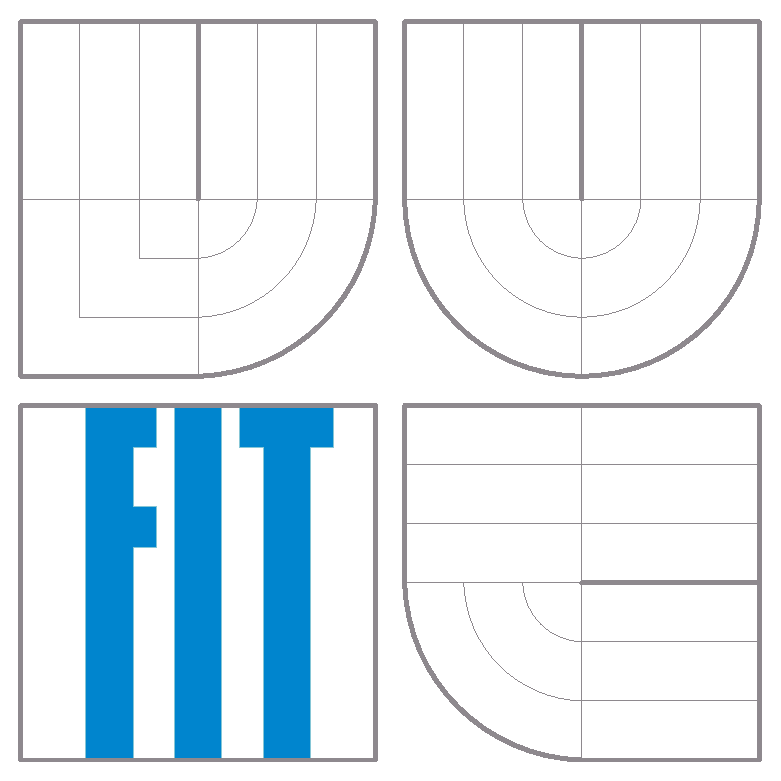
\includegraphics[height=5cm]{logo.eps}~\\
\vfill
{\LARGE Tvorba uživatelských rozhraní}\\
\medskip
{\Huge Elektronický kalendář}\\
\end{center}
\vfill
\begin{minipage}{0.5\textwidth}
\begin{flushleft}
{\Large \today}
\end{flushleft}
\end{minipage}
\begin{minipage}{0.5\textwidth}
\begin{flushright}
{\Large
Michal Duban, xduban01\\
Marko Fábry, xfabry01\\
\medskip
Jan Wrona, xwrona00
}
\end{flushright}
\end{minipage}
\end{titlepage}

\tableofcontents
\clearpage

%%%%
\section{Úvod} \label{uvod}
%%%%
Ačkoli zadání specifikuje tvorbu celé aplikace, hlavním cílem projektu je navrhnout, zrealizovat, otestovat a vyhodnotit především uživatelské rozhraní. Proto je kladen důraz především na jednoduchost, rychlost, přehlednost a intuitivnost ovládání spolu s čistým a vzdušným vzhledem. Z důvodu menší priority kladené na programovou funkčnost a omezených časových možností se proto může zdát program místy funkčně nekompletní a uživateli mohou chybět některé specifičtější úkony či možnosti.

\subsection{Popis zadání}
Navrhněte aplikaci, která by umožnila vykreslit kalendář přímo na pozadí plochy či do aktuálního obrázku na ploše. Kalendář by měl umožňovat různé typy zobrazení (týdenní, měsíční, vybraný počet týdnů a měsíců dopředu, různá poloha na ploše) a zvýraznit současný den, týden, měsíc a číslo týdne dle kalendáře. Kalendář by měl být připraven na případné zobrazování svátků. Zaměřte se zejména na vzhled rozhraní a intuitivnost a efektivitu ovládání.

%%%%
\section{Analýza} \label{analyza}
%%%%
Před začátkem tvorby aplikace jsme provedli průzkum aplikací, které podobnou funkčnost již implementují. Všichni jsme měli zkušenost s online kalendářem společnosti Google a až na drobné výjimky jsme shodli na jeho vysoké kvalitě co se týče ovladatelnosti i funkčnosti. Tento kalendář ale funguje (mimo mobilní zařízení) pouze jako webová aplikace což je od cílové platformy tohoto projektu (plocha grafického desktopového prostředí) poněkud vzdálené. Hledali jsme tedy dále mezi desktopovými aplikacemi a nalezli a vyzkoušeli jsme aplikace Samurize\footnote{\url{http://www.samurize.com/}} a Rainlendar\footnote{\url{http://www.rainlendar.net/}}. Oba tyto programy jsou zaměřeny podobným směrem jako tento projekt nicméně každý má jiné možnosti a specifika. Ani jeden z nich ale plně nevyhovuje zadání a proto se po analýze dalo říci, že budeme tvořit aplikaci ve své kategorii jedinečnou.

%%%%
\section{Návrh a popis rozhraní} \label{navrh}
%%%%
Jak je zmíněno v analýze, všichni jsme ovlivněni používáním online Google kalendáře, jsme zvyklí na jeho způsob zobrazování a ovládání. Přesto jsme se ale nespokojili s jeho jednoduchým okopírováním a určité prvky jsme navrhli jinak. Lze ale říci že způsob zobrazení týdne a měsíce Google kalendářem se pro nás stal referenčním především proto, že je takové rozložení políček dne/hodiny široce používané a jeho změna by nutila uživatele si zvykat na již zažitou věc (pokud má uživatel předchozí zkušenosti s elektronickým kalendářem) čímž by zajisté utrpěla intuitivnost. Tímto ale inspirace u Googlu končí, protože desktopová platforma nabízí jiné a širší možnosti ovládání, zobrazování či nastavování a některé z nich jsou přímo vyžadovány.

\subsection{Koncepce oken}
Tato subsekce je zde umístěna z důvodu ne úplně běžné koncepce programu. Běžný program s grafickým uživatelským rozhraním (dále GUI) po spuštění zobrazí hlavní okno aplikace přes všechny doposud otevřené okna (bude navrchu), ze kterého se spolu s uživatelskou interakcí mohou zobrazovat další okna či dialogy. Naše koncepce funguje odlišně. Program po spuštění hlavní rodičovské okno (pohled) aplikace nezobrazí na vrchu ale naopak pod všemi zobrazenými okny, co nejblíže systémové ploše. Zároveň se zobrazí ikona v hlavním panelu (tray). Proč tomu tak je a jaký tyto prvky mají význam je vysvětleno následovně.

\subsection{Hlavní pohled}
Jedná se o nejdůležitější část celé aplikace, která zajišťuje zobrazení buď jednoho týdne nebo jednoho měsíce na pracovní ploše.  Ačkoli se programově jedná o typické obdélníkové okno, rozhodně tomu tak není co do vzhledu ani použití. Protože našim cílem bylo vytvořit aplikaci, která bude typicky běžet po celou dobu běhu počítače, je důležité aby nepůsobila rušivě. Proto je tento pohled vždy zobrazen nejníže (pod všemi ostatními okny) a není možné toto chování uživatelem změnit. Při návrhu jsme mysleli také na to, že uživatel na ploše může mít ikony, widgety či prostě chce vidět obrázek na pozadí. Přidáním částečné transparentnosti tomuto pohledu docílíme viditelnosti ikon i pozadí, ale naskytne se problém se zasíláním zpráv klávesnice a myši nikoliv objektům na ploše ale našemu hlavnímu pohledu. Řešením je tzv. click-through vlastnost okna, která zajišťuje předávání událostí od myši objektům pod naším oknem, ikony tedy budou plně funkční.

Součtem těchto atributů vznikne pohled na aplikaci, která uživatele v ničem neomezuje, neruší a zároveň efektivně využívá pracovní plochu ať už celou či jenom její část. Obsah tohoto pohledu je zřejmý z názvu projektu. Je jím kalendář buď v týdenním či měsíčním zobrazení.

Grafický návrh týdenního kalendáře je vidět na obrázku č. \ref{fig:week}. Dny v týdnu jsou umístěny na horizontální ose, hodiny od 0 do 23 jsou umístěny na vertikální ose. Buňka vlevo nahoře je využita určena pro vypsání čísla aktuálně zobrazeného týdne. Většinovou část tvoří tabulka do které se budou programově zobrazovat události. Jemným barevným rozdílem jsou odlišeny sudé a liché hodiny pro snadnější orientaci, jednotlivé políčka tabulky jsou odděleny malým prázdným místem (spacing) což oproti použití ohraničení (border) návrhu dodává vzdušnost.
\begin{figure}[h]
    \centering
    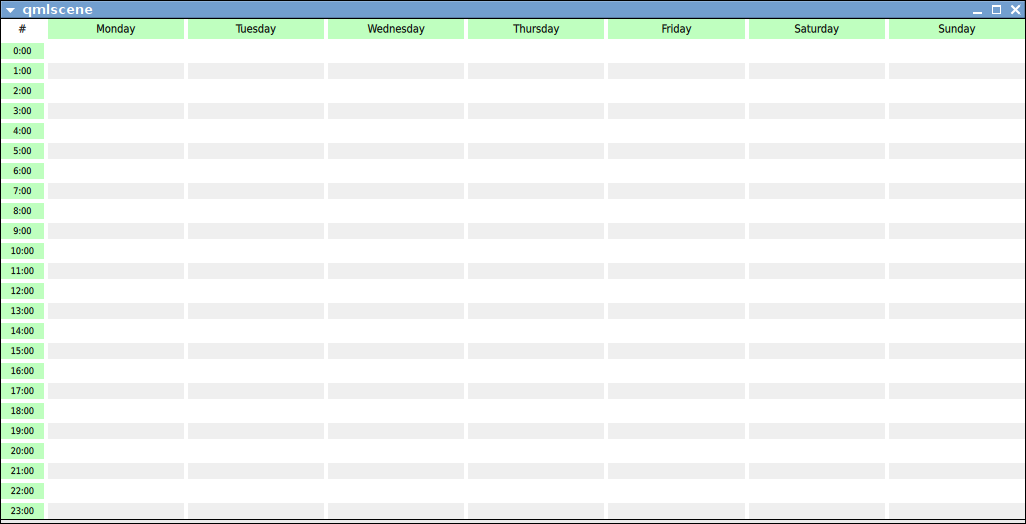
\includegraphics[width=\textwidth,height=\textheight,keepaspectratio]{week.png}
    \caption{Týdenní pohled}
    \label{fig:week}
\end{figure}

Měsíční zobrazení č. \ref{fig:month} je graficky sjednocené se zobrazením týdne. Dny od pondělí do neděle jsou opět zobrazeny na horizontální ose, týdny jsou zobrazeny na ose vertikální. Buňky prvního sloupce zleva jsou určeny pro vypsání čísla týdne. Opět je použit spacing mezi buňkami.
\begin{figure}[h]
    \centering
    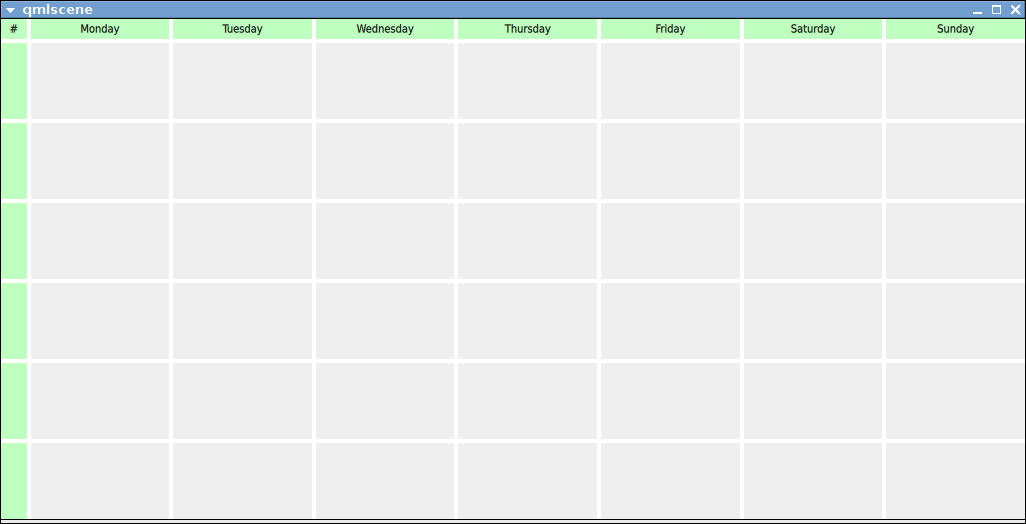
\includegraphics[width=\textwidth,height=\textheight,keepaspectratio]{month.png}
    \caption{Měsíční pohled}
    \label{fig:month}
\end{figure}

\subsection{Nastavení}
Veškerá nastavení se vyvolávají přes klik pravým tlačítkem na dříve zmiňovanou ikonu v oblasti tray hlavního panelu. Tento klik vyvolá menu, které nabízí možnosti ukončení aplikace, zobrazení a schování hlavního pohledu, změnu velikosti hlavního pohledu, změnu týdenního a měsíčního pohledu, změnu aktuálně zobrazeného data a konečně zobrazení okna pro editaci kalendářů. Editační okno obsahuje možnosti jako přihlášení do online Google účtu, zobrazení kalendářů uživatele (lokálních i vzdálených) a při výběru kalendáře jsou zobrazeny naplánované události. Samozřejmostí jsou možnosti jako přidání, editace a smazání kalendáře či události. Při nutnosti zadání data (počátek a konec události) má uživatel možnost zadání tohoto data textem či výběrem z kalendáře.

\subsection{Ovládání}
Názvy položek menu a tlačítek jsme volili tak, aby z něj byla funkce co nejjasnější. Při testování jsme objevili funkci, kterou uživatelé obtížně ovládali, proto je nutné ji zavést do dokumentace. Jedná se o uložení pozice a velikosti zobrazení hlavního pohledového okna, které se vyvolává přes nabídku z ikony v tray. Kromě opětovného vyhledání tlačítka v nabídce existuje možnost uložení stiskem pravého tlačítka na myši.
%%%%
\section{Implementace} \label{implementace}
%%%%
Aplikace byla od počátku vyvíjena jako multiplatformní desktopová aplikace. Na základě tohoto předpokladu jsme také zvolili příslušný GUI toolkit. Hned na začátku ale musím zmínit, že tento bod není dotažen do konce a pro totožnou funkci na různých grafických desktopových prostředích (cílem jsou především Windows 8, Gnome a Unity) je potřeba ještě nějaká práce. Nejdetailněji je aplikace testovaná na odladěná na x86\_64 systému s OS Windows 8.1. Dále v této sekci budou popsány a zdůvodněny implementační detaily aplikace jako jsou použité programovací jazyky, toolkity a převzaté knihovny.

\subsection{Programovací jazyk}
Funkční část (model, controller) je psaná v programovacím jazyce C++. Tento jazyk je mezi čitateli této sekce dokumentace pravděpodobně dobře znám a není ho třeba představovat. Použití právě tohoto jazyku je odůvodněno volbou GUI toolkitu jakožto knihovny pro C++.
\subsection{GUI toolkit}
Jako GUI toolkit jsme si zvolili Qt. Důvody volby této knihovny nejen pro tvorbu GUI je jeho multiplatformnost, vysoká rozšířenost ale také jeho výuka v kurzu ITU. Nutno ovšem uvést, že jeho multiplatformnost při specifičtějších požadavcích na zobrazení není vždy dokonalá. Jak jsme si sami ověřili, místy je nutné používat preprocesorová makra závislá na operačním systému. Jako příklad můžu uvést metodu {\texttt showMaximized()} třídy {\texttt QDeclarativeView}, která by měla maximalizovat okno. Na Windows 8.1 ale způsobuje zobrazení okna na  celou obrazovku (fullscreen), proto jsme museli využít funkcí {\texttt WinAPI}. Mimo jiné využíváme třídy tohoto toolkitu ke zpracování serializačního formátu JSON, který je použit pro perzistentní data kalendářů ale také pro vyměňování dat s Google API (sekce \ref{sprava}).

Zobrazovací část (viewer) je řešena dvěma jazyky a způsoby. První z nich je využití programu Qt Designer, který umožňuje vizuální tvorbu prvků uživatelského rozhraní. Jeho výstupem je XML popisující tyto vizuálně vytvořené prvky. Tento způsob je použit u okna pro editaci kalendářů a jeho dialogových oken. Druhým přístupem, poněkud sofistikovanějším, je použití deklarativního jazyka QML založeného na JavaScriptu. QML je přednostně určen pro tvorbu uživatelských rozhraní a je ti část toolkitu Qt, která se jmenuje \texttt{QtQuick}. Tento přístup je použit u hlavního pohledu pro týden i měsíc. Na jeho kvalitu byl kladen velký důraz. Veškeré prvky dynamicky dle velikosti okny mění svou velikost ve správném poměru, velikost textu je také dynamicky měněna s cílem dobré čitelnosti i v malých buňkách. Text se také automaticky zalamuje.

Několik nejpoužívanějších Qt tříd:
\begin{itemize}
  \item {\texttt QDeclarativeView} - zobrazování QML
  \item {\texttt QMainWindow} - zobrazování ostatních oken
  \item {\texttt QJson} - práce s JSON
\end{itemize}

\subsection{Správa kalendářů a událostí} \label{sprava}
V této části se program dělí na dvě části. První je pouze lokální úložiště na klientském stroji. Druhou možností je Google Calendar API, které umožňuje vyvíjet klientské aplikace, které mohou vytvářet, editovat a mazat události či celé kalendáře. Samozřejmostí je možnost si stáhnout kalendář. Pro uživatele to nabízí možnost se přihlásit přes svůj Google účet (lze ho z aplikace i vytvořit) a získat tak nové možnosti propojením desktopové aplikace se svými kalendáři v cloudovém úložišti přístupném z internetu. Tato funkcionalita je nad rámec zadání tohoto projektu a ačkoli její implementace stála spoustu času, v době psaní dokumentace nebyla zcela dokončená (ze vzdáleného kalendáře nelze zobrazovat události do hlavního okna na ploše).

\subsection{Převzaté zdroje}
Kromě Qt je v projektu využita knihovna {\texttt qt-oauth-lib}\footnote{\url{https://code.google.com/p/qt-oauth-lib/}}, což je knihovna využívající Qt vytvořena společností Integrated Computer Solutions, Inc. poskytující autentifikaci a autorizaci OAuth2.0 potřebnou pro Google API šířená pod licencí GNU Lesser GPL. Bylo ovšem nutné kvůli změně ze strany Google tuto knihovnu pozměnit, proto se vyskytuje mezi odevzdanými zdrojovými texty.

Dále jsme využili volně dostupnou ikonu kalendáře\footnote{\url{http://www.iconarchive.com/show/icons8-metro-style-icons-by-visualpharm/Very-Basic-Calendar-icon.html}}.

%%%%
\section{Testování rozhraní} \label{testovani}
%%%%
Tato sekce popisuje návrh, popis, průběh, výsledky a vyhodnocení testování vytvořeného GUI.
\subsection{Návrh}
Průběh testů je rozdělen do čtyř bodů:
\begin{enumerate}
\item uživatel vidí aplikaci poprvé, je mu vysvětleno k čemu slouží a její základní princip (nic co se ovládání týče)
\item postupně jsme uživateli zadali úkoly a měřili čas jejich provedení
\item dali jsme uživateli možnost si aplikaci prozkoumat a zeptat se na nejasnosti
\item bod 2. jsme opakovali v jiném pořadí
\end{enumerate}
Úkoly:
\begin{description}
    \item[a)] vytvořit nový kalendář a vložit do něj událost
    \item[b)] nalézt tlačítko pro změnu velikosti a pozice zobrazeného pohledu
    \item[c)] zobrazit následující týden
\end{description}

\subsection{Výsledky}
Výsledky jsou uvedeny v tabulce \ref{tab:vysledky}.
\begin{table}[h]
    \begin{center}
    \begin{tabular}{| c | c | c | c || c | c | c |}
    \hline
     & \multicolumn{3}{|c||}{Pokus č. 1} & \multicolumn{3}{c|}{Pokus č. 2}\\
    Uživatel & a & b & c & a & b & c \\
    \hline
    Hana D. & 69 & 9 & 17 & 34 & 4 & 10 \\
    Martin D. & 32 & 5 & 11 & 28 & 3 & 7 \\
    Martin P. & 53 & 10& 19 & 31 & 7 & 6 \\
    Michal K. & 71 & 5 & 12 & 38 & 4 & 7 \\
    Tomáš P. & 66 & 7 & 18 & 40 & 5 & 8 \\
    Vít M. & 60 & 7 & 12 & 25 & 6 & 9 \\
    Gabina J. & 51 & 9 & 17 & 34 & 8 & 6 \\
    Petr C. & 71 & 8 & 17 & 37 & 4 & 10 \\
    Bianka F. & 74 & 8 & 16 & 29 & 6 & 14 \\
    \hline
    Průměr: & 60.77 & 7.55 & 15.44 & 32.88 & 5.22 & 8.55\\
    \hline
    \end{tabular}
    \caption{Tabulka výsledků}
    \label{tab:vysledky}
    \end{center}
\end{table}

\subsection{Vyhodnocení}
Dlouhá průměrná doba u prvního pokusu testu a) je způsobena především dobou hledání ikony kalendáře v liště. Časté byly pokusy kliků na kalendář levým či pravým tlačítkem myši. Dále kliknutí na ikonu levým tlačítkem myši, které také nemá přiřazenou žádnou akci. Tato nenápadnost běžící aplikace se tak při prvním použití projevila spíše negativně. Testy b) a c) už díky uživatelově znalosti ikony byly časově podstatně kratší.

Opakování testů mělo hlavní důvod zjistit rozdíl mezi prvním použitím aplikace (intuitivnost) a následným rutinním používáním (jednoduchost, zapamatovatelnost ovládacích prvků). Tento rozdíl se ukázal jako výrazný, doba se navíc po dalším používání bude pravděpodobně ještě zmenšovat.

Testy nebyly prováděny v jednu dobu, tudíž verze aplikace se během jednotlivých testování lišily. Dají se ovšem považovat za dostatečně vypovídající proto, že v době testování se neprováděly už žádné výraznější změny v ovládání.

\subsection{Připomínky testerů}
Rozhraní je v angličtině nepěkné barvy, nemožnost jejich změny, kopírování kódu po přihlášení ke Google účtu, dlouhá odezva při operacích se vzdáleným kalendářem.

%%%%
\section{Prostor k zlepšení a známé nedostatky}
%%%%
\begin{itemize}
    \item Zobrazování událostí v současné době nepodporuje vykreslování Google kalendářů a paralelních událostí v zobrazení týdne.
    \item Celodenní události by šly řešit lépe.
    \item Uživatel by měl mít možnost změnit kalendáři barvy.
    \item Měla by existovat možnost nastavení české lokalizace.
    \item Plná podpora pro jiné operační systémy.
\end{itemize}

%%%%
\section{Závěr}
%%%%
Při prvotním plánování a analýza jsme přecenili své schopnosti a časové možnosti, chtěli jsme implementovat příliš mnoho funkčnosti. Tento fakt jsme si časem uvědomili a přizpůsobili (zjednodušili) jsme návrh. Stejná tendence lze vidět i na odevzdaných dokumentech plán a revize.

Značné zjednodušení návrhu uživatelskému rozhraní neuškodilo a podařilo se nám vytvořit zajímavou aplikaci s uživatelským rozhraním, které splňuje náš původní záměr - přehlednost, intuitivnost, praktičnost. Výsledky testů ukázaly, že při prvním použití může uživatel tápat, což je způsobeno záměrnou nenápadností běžící aplikace.
\end{document}
